%*
%* Seven Kingdoms: Ancient Adversaries
%*
%* Copyright 1997,1998 Enlight Software Ltd.
%* Copyright 2018 Timothy Rink
%*
%* This program is free software: you can redistribute it and/or modify
%* it under the terms of the GNU General Public License as published by
%* the Free Software Foundation, either version 2 of the License, or
%* (at your option) any later version.
%*
%* This program is distributed in the hope that it will be useful,
%* but WITHOUT ANY WARRANTY; without even the implied warranty of
%* MERCHANTABILITY or FITNESS FOR A PARTICULAR PURPOSE.  See the
%* GNU General Public License for more details.
%*
%* You should have received a copy of the GNU General Public License
%* along with this program.  If not, see <http://www.gnu.org/licenses/>.
%*
%*

\chapter{Harbors and Ships}

\begin{wrapfigure}{l}{0.2\textwidth}
	\vspace{-20pt}
	\begin{center}
		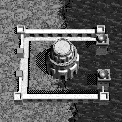
\includegraphics[width=0.2\textwidth]{Iharbor}
		\\ Habor
	\end{center}
	\vspace{-20pt}
\end{wrapfigure}

Depending upon the geographic situation of your Empire, Harbors and the ships that are built in them could come to have an overriding importance to your survival.

From an isolated stretch of land or from an island, it will only be by sea that you will be able to carry on trade or to expand your Empire.

% IS THIS CENTERED? PROBABLY THE ABOVE IMAGE IS MAKING IT ENTER A WRAPFIGURE

\begin{center}
	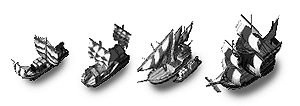
\includegraphics[width=0.7\linewidth]{Iships}
	\\ Trader Transport Caravel Galleon
\end{center}

\section{Traders}

These unarmed vessels may carry a cargo of raw materials or of finished goods of up to 250 units. They may not carry Soldiers or Peasants.

There is no need to research Traders. You begin the game with the knowledge of their construction.

\section{Transports}

These unarmed vessels carry no goods, only people or Weapons. Their capacity is nine People or Weapons or a combination of the two. While on Transports, Weapons may not be fired either offensively or defensively.

There is also no need to research Transports.

\section{Caravels}

\index{caravels}

Caravels are capable of carrying both goods and military units. Each Caravel comes with pre-mounted Cannon that may not be removed from the Ship. Other Weapons placed on board may not be used for the Ship’s defense.

\subsection{On-Board Leadership}

If you have any Soldiers on board your Caravel or your Galleon (Below), the one with the highest Leadership Level will direct the Ship’s Cannon. If his Leadership Level is 100, for example, your Cannon’s fire-power will be double that of a Cannon without leadership.

The Caravel’s capacity is nine People or Weapons or a combination of the two. Its goods carrying capacity is, as with the Traders, 250 units. Caravels may not be researched until you have finished researching Cannon.

\section{Galleons}

Galleons, like Caravels, are capable of carrying both goods and military units. Each Galleon is built with pre-mounted Cannon that may not be removed from the Ship. As with the Caravel, other Weapons placed on board may not be used for the Ship’s defense.

The Galleon’s capacity is, as with the Caravel, nine People or Weapons, or a combination of the two. Its goods carrying capacity is double that of Traders and Caravels. And, although you will find that Galleons are slower than the smaller Caravels, they do pack more powerful Cannon and can take more punishment before sinking. Galleons may not be researched until you have finished researching Caravels.

\section{Damaged Ships and Injured Sailors Contents}

\index{damaged ships}

Damaged Ships will slowly repair themselves if they are not moving and will repair twice as fast in Harbors. Any injured Soldiers on ships will slowly regain their health whether the Ship is moving or not. They will regain their health twice as fast if their Ship is in Harbor.

All Harbors have a capacity of four ships.

\begin{center}
	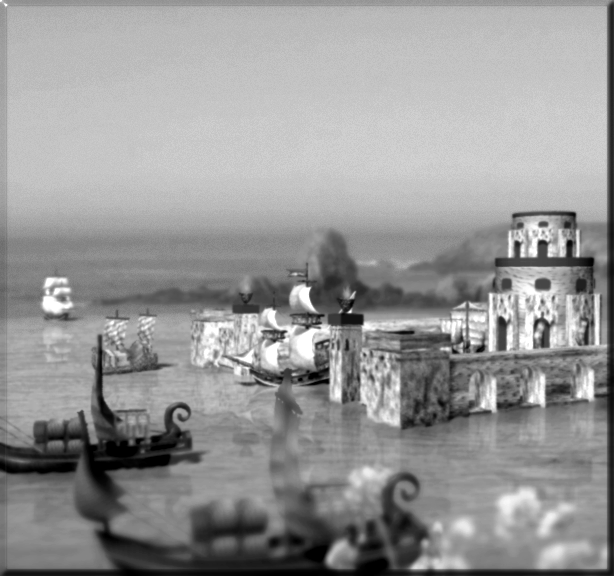
\includegraphics[width=0.7\linewidth]{Aharbor}
\end{center}

\section{Conducting Seaborne Trade}

\subsection{Linking Harbors to Sources of Goods}

For a Harbor to function as a trading port, it must be Linked directly to a Market, Factory, or Mine. If a Market, then that Market should be receiving goods from somewhere, either by direct Link or by Caravan.

With these Links, Finished Goods from the Market or Factory and Raw Materials from the Market or Mines will be automatically sent to the Harbor where they will be picked up by Traders that call there.

\subsection{Building Ships for Trade}

\index{building!ships} You will begin the game with the technological ability to build Traders, so there will be no need for you to research them. Later, as your technology progresses, you will be able to build Caravels and Galleons to more efficiently and safely conduct seaborne trade.

\begin{wrapfigure}{r}{0.1\textwidth}
	\vspace{-20pt}
	\begin{center}
		
\includegraphics[width=0.1\textwidth]{Tshipmake}
	\end{center}
	\vspace{-20pt}
\end{wrapfigure}

Caravels and Galleons may, of course, also be used solely for purposes of war. To build a Ship, select the Harbor and then \textbf{Click} on the \textbf{Build Ship Tile}.

\begin{wrapfigure}{r}{0.5\textwidth}
	\vspace{-20pt}
	\begin{center}
		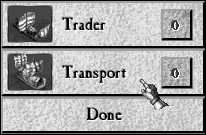
\includegraphics[width=0.4\textwidth]{Iship_begin}
	\end{center}
	\vspace{-20pt}
\end{wrapfigure}

You will then see a selection of Ships that you will be able to build with your present technology. \textbf{Click} on the Ship that you want to build.

You may build more than one Ship at a time, though if the Harbor is full (maximum four Ships), production will cease until there is space made for them.

To build multiple ships, \textbf{Click} on the number on the right until it shows the number that you want to build. \textbf{Right-Click} on the number to lower it.

When you are finished, \textbf{Click} on the \textbf{Done Button}. The Ships will be built as you order.

\begin{wrapfigure}{r}{0.5\textwidth}
	\vspace{-20pt}
	\begin{center}
		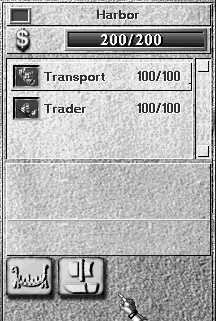
\includegraphics[width=0.4\textwidth]{Iharborinfo}
	\end{center}
	\vspace{-20pt}
\end{wrapfigure}

When the Ship is finished it will appear in the harbor where you have the choice of leaving it there or of setting sail. To set sail, \textbf{Click} on the desired Ship and then \textbf{Click} on the \textbf{Set Sail Tile}. \textbf{\textit{See Below}}.

% "See Below" bf and it? weird. check similar usage

\clearpage

\subsection{Setting Sail}

\begin{wrapfigure}{r}{0.1\textwidth}
	\vspace{-20pt}
	\begin{center}
		
\includegraphics[width=0.1\textwidth]{Tsail}
	\end{center}
	\vspace{-20pt}
\end{wrapfigure}

When you wish to send ships out of the Harbor, \textbf{Click} on the desired Ship and then \textbf{Click} on the \textbf{Set Sail Tile}. Your Ship will then exit the Harbor and await further commands.

\begin{center}
	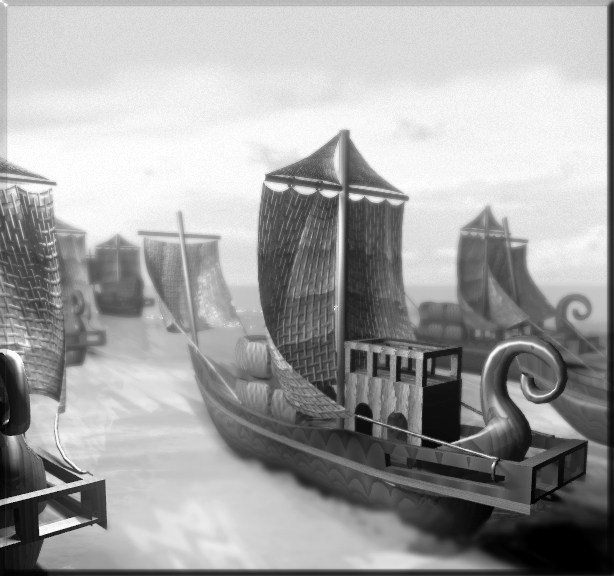
\includegraphics[width=0.7\linewidth]{Aship}
\end{center}

\subsection{Setting Trade Routes and Cargo}

\begin{wrapfigure}{r}{0.1\textwidth}
	\vspace{-20pt}
	\begin{center}
		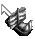
\includegraphics[width=0.1\textwidth]{Bship}
	\end{center}
	\vspace{-20pt}
\end{wrapfigure}

Setting the seaborne trade routes and Ship loads is exactly the same as setting the Caravan routes, except that when a Ship is selected, you must use the Ship and Arrow Cursor (Right) to \textbf{Click} on either your other Harbors or on the Harbors of Kingdoms with which you have a Trade Treaty.

\begin{wrapfigure}{r}{0.5\textwidth}
	\vspace{-20pt}
	\begin{center}
		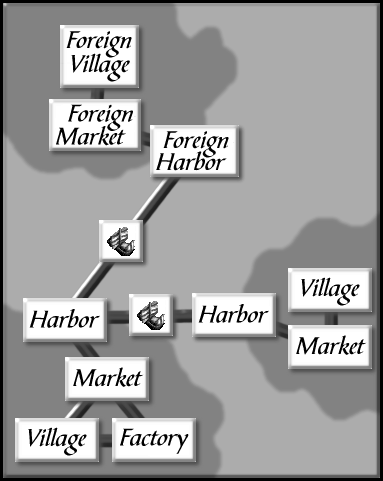
\includegraphics[width=0.4\textwidth]{Iharbortradesit}
	\end{center}
	\vspace{-20pt}
\end{wrapfigure}

When a route is set, your Ship will automatically sail back and forth between those Harbors, picking up and delivering Finished Goods and Raw Materials.

You will be able to set the cargo for the Ships in the same way as you set the loads for the Caravans.

Make sure when sending your Ships to pick up goods from foreign Harbors that those Harbors have Markets Linked to them.

You may \textbf{\textit{not}} pick up goods from a foreign Factory or Mine that is Linked to a foreign Harbor. Only their Ships will have that ability.

As with Caravans and foreign Markets, your Ships may \textbf{\textit{not}} drop off goods in foreign Harbors. They may only pick up goods that are for sale in a Linked Market.

Your goods will be sold when foreign Ships call at your Harbors.

\subsection{Controlling your Ships}

\index{controlling ships}

\begin{wrapfigure}{r}{0.5\textwidth}
	\vspace{-20pt}
	\begin{center}
		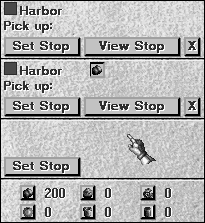
\includegraphics[width=0.4\textwidth]{Ishipinfo}
	\end{center}
	\vspace{-20pt}
\end{wrapfigure}

There are two modes of control for your Ships of Trade. The default mode is T (Trade), where the Ships will continuously sail their trading route.

If for any reason you wish to take your ship out of its set route, without losing all of the routing programming, \textbf{Click} on the \textbf{T Button} to change it into an C (Control). In this mode, you will be able to direct your Ship either to a safe area or into battle.

By \textbf{Clicking} on the \textbf{Units} or \textbf{Goods Buttons}, you will be able to view either the Soldiers and Weapons on board or the cargo and trading routes that you have set.

\section{War on the High Seas}

\subsection{Attacking with Ships}

Caravels and Galleons may be used to attack any other ship or any land or airborne target that is within range.

Remember that if your Caravel or Galleon is on a trading route and you wish to use it for battle, you should \textbf{Click} on the \textbf{T (Trade) Button} — changing it into the \textbf{C (Control) Button}. After the battle, \textbf{Click} on the \textbf{C Button} again. It will change back into a T and your Ship will resume its trading route.

Attacking a Trader will have the same effect as attacking a Caravan on land. Although you may cut off your opponent’s trade, attacking a civilian vessel will damage your Reputation.

Additionally, if one of your Traders is sunk by an enemy, your Reputation will also suffer because of your inability to protect your civilians.

\subsection{Loading Soldiers and Weapons onto Warships}

\begin{wrapfigure}{r}{0.5\textwidth}
	\vspace{-20pt}
	\begin{center}
		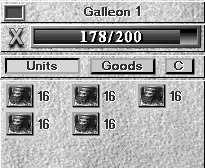
\includegraphics[width=0.4\textwidth]{Igalleonfull}
	\end{center}
	\vspace{-20pt}
\end{wrapfigure}

To load Soldiers and Weapons for transport onto a Ship, \textbf{Group Select} the intended units and then \textbf{Right-Click} on the Ship. When \textbf{Right-Clicked}, the Ship will move to the shore and the Soldiers and Weapons will board.

To view the units that you have just loaded, \textbf{Click} on the \textbf{Units Button}.

\subsection{Unloading Warships}

Move your Ship up onto the shore and make sure that the \textbf{Units Button} has been \textbf{Clicked}. Now, \textbf{Right-Click} on the Soldier or Weapon that you want to take off of the Ship. That Soldier or Weapon will then be off-loaded onto the beach.

\begin{wrapfigure}{r}{0.1\textwidth}
	\vspace{-20pt}
	\begin{center}
		
\includegraphics[width=0.1\textwidth]{Tdisembark}
	\end{center}
	\vspace{-20pt}
\end{wrapfigure}

To unload the entire Ship’s company onto the beach, you must \textbf{Click} the \textbf{Disembark Tile}. When you do so, your Ship will quickly empty itself of its Soldiers and Weapons.